\documentclass[12pt]{article}
%Gummi|065|=)
%This Latex file is meant to be added upon and edited as seen fit by future students.
%In the interest of version control and posterity please preserve the source code of this and any other final versions with the SSC, and save any future documentation as a new version.

%Editors:
% v2025: Nathan Ryan (University of Illinois Urbana-Champaign). Assisted by Eileen Cullen and Chloe Martin (ANS Conference Staff and awesome people).
% v2017: Matthew Jasica (University of Wisconsin). Assisted by Forrest Shriver (University of Florida), Kalin Kiesling (University of Wisconsin) and Sarah Camba Lynn (Texas A&M)
%Pre-version 2017 edits that directly influenced this write-up go back at least as far as 2010, but lack a source file or documentation of editors. Version 2017 merely marks the first time this manual was documented as a Latex file.

%Changelog: (future editors may add on to, modify, or simplify as seen fit)
% Updated 05-18-2025 by Nathan Ryan (incorporate feedback from Eileen Cullen and Chloe Martin)
% Updated 03-12-2025 by Nathan Ryan (grammatical edits)
% Updated 03-05-2025 by Nathan Ryan (add automatic compilation as an artifact)
% v2017, 07-20-2017, Final push
% Updated 07-20-2017 by MJ w/ final edits and markup.
% Updated 07-11-2017 by MJ w/ revisions from K Kiesling and consistency
%   -Prior red text indicating changes from 2013 version removed. New red color reflects changes since April 16 version
% Updated 06-04-2017 by MJ, slight formatting tweaks for consistency between documents
% Updated 05-20-2017 by MJ, added title page
% Updated 05-09-2017 by Matthew Jasica (minor edits only)
% Updated 04-16-2017 by Forrest Shriver

\usepackage[utf8]{inputenc}
\usepackage[margin=1in]{geometry}
\usepackage{enumitem}
\usepackage{graphicx}
\usepackage{color}
\usepackage{textcomp}
\usepackage[colorinlistoftodos]{todonotes}
\usepackage{tocloft}
\usepackage[colorlinks=true, urlcolor=blue, linkcolor=black]{hyperref}

%\renewcommand\cftchapafterpnum{\vskip6pt} %adjust ToC spacing
\renewcommand\cftsecafterpnum{\vskip6pt}
\setlength{\parindent}{0pt}
\setlength{\parskip}{1em}

\title{\textbf{Student Conference Proposal Guidelines}}
\author{American Nuclear Society}
\date{}
\begin{document}

\newcommand{\redcolor}{\textcolor{red}}

\begin{titlepage}
\vspace*{2cm}
\centering
{\Huge\bfseries Student Conference Proposal Manual\par}
%\vspace{1cm}
%\textit{\LARGE American Nuclear Society Student Sections Committee}

\vspace{2cm}
\rm{\Large Revised May 2025\par }

\vfill

\includegraphics[scale=0.75]{SSClogo.png}
\end{titlepage}

%\maketitle

\clearpage
{\hypersetup{linkcolor=black}
\tableofcontents
}

\newpage

\section{Introduction}

ANS student sections interested in hosting the ANS Student Conference can apply to do so by drafting a proposal and submitting it to the ANS Student Sections Committee (SSC). This document was developed by past organizers of the ANS Student Conference and the ANS Conference Staff to provide prospective conference hosts with information and expectations regarding the ANS Student Conference proposal process. The current document is an official and primary source of instruction on how to draft and submit a student conference proposal. An additional resource, the Student Conference Planning Manual, is available that goes into more detail about planning a conference \emph{after} a proposal is selected. However, the Planning Manual is still highly recommended reading for sections wishing to submit a proposal. For additional information on the ANS Student Conference and the ANS Student Conference proposal processes, visit the SSC website, \href{http://students.ans.org/}{http://students.ans.org/}, or contact the SSC at \href{mailto:sscChair@gmail.com}{sscChair@gmail.com}.


The ANS Student Conference is held every year in the spring and is organized  by the student members of the ANS in partnership with the ANS National COnferences Department. Conference participants include students, professors, professionals, and recruiters from all fields of nuclear science and technology. The conference focuses on the professional development of student participants. Professional development opportunities have historically taken the form of guest speakers, student research presentations, workshops, tours, networking, and mentorship. The conference also highlights the breadth or scope of nuclear science and engineering to the attendees by bringing together the various specialties and sub-specialties emphasized at the different schools in attendance. Another aim of the conference is to illustrate the idea a professional meeting where students and professionals can exchange ideas, information, and build professional relationships.

These conferences are attended by approximately 450 students, 150 professionals, and dozens of universities and companies. The conference has become a large operation which requires extensive staff and complex logistics. The calendar time required to set up the conference is relatively long for a student endeavor: approximately 6 months to prepare a proposal and approximately 18 months to execute the proposal. Because this commitment is longer than one school year, conference planning can be severely hindered by graduation of the students behind proposal submissions, if not properly anticipated.

Sections submitting for the first time should not be discouraged if their proposal is not accepted. Often, initial proposals will not be chosen, as a proposal needs at least one round of feedback from reviewers before being considered fully-prepared. The recommendation in such a situation is to take the feedback received and make efforts to improve accordingly, with the goal of being accepted the following year.

\subsection{Outline of Proposal Process}
\begin{enumerate}
\item{Read this document}
\item{Visit the \href{http://students.ans.org/student-conferences/}{Student Conference} page of the Student Sections Committee (SSC) website. This site contains links to past conference proposal documents, past conference websites, and other information.}
\item{Read the conference proposal Judges’ Evaluation Worksheet posted on the \href{http://students.ans.org/student-conferences/}{SSC website}. It is worth checking periodically for any updates to this worksheet.}
\item{Visit past and current conference websites, if available. Pay particular attention to past conference programs, which may be available through the websites (or past Chairs). Internet searches of ``20XX ANS Student Conference” may be helpful.}
\item{Confirm the student section's ``Good Standing" status within ANS. The section should be active enough to supply the staff and time to host the conference. The \href{http://students.ans.org/section-standing/}{Section Standing} page of the SSC website lists the standing of each section. Sections not in good standing should follow the instructions provided on the website to fix this. Sections not in good standing for some time should consider this is a warning sign that they may not yet be ready to host.}
\item{Begin gathering information about the practical aspects of hosting a conference. Specific details are provided later in this document. Proposal committees are strongly encouraged to contact past conference Chairs---see Section \ref{sec:points_of_contact}. \textbf{Recommended date: May 1st}}
\item{Send as many section members affiliated with the proposal as possible to any student conferences or national meetings that occur while preparing the proposal.}
\item{Contact the \href{mailto:sscChair@gmail.com}{SSC Chair} and inform him/her of the section’s intent to prepare a proposal. By doing so, there is no implied commitment by the section to submit a proposal. However, this ensures that proposal committee will receive timely notification of any changes that impact the application process. \textbf{Recommended date: August 1st}}
\item{Write the formal student conference proposal document. \textbf{Recommended date: August 1st}}
\item{Submit the conference proposal to the SSC Chair before the deadline posted on the SSC website. \textbf{Deadline: October 1st}}
\item{Wait for the SSC’s decision to be announced at the ANS Winter Meeting that November. Send at least a few representatives, in particular any Chair(s) of the proposal. Accepted proposal Chair(s) can start talking to ANS National and the SSC about the planning process. For sections that are not selected, this is a great opportunity to review what can be improved, removed, or added for the next proposal.}
\end{enumerate}

\subsection{Proposal Objective}
An ANS Student Conference proposal should convince a panel of judges of the submitting student section’s ability to host a successful conference. These judges are members of the SSC, including both past conference Chairs (for more information on the Judging Committee, selection rules are available for download on the \href{http://students.ans.org/student-conferences/}{SSC website}).
There are two main
components to a successful conference:
\begin{enumerate}
\item{Sound leadership and vision}
\item{A sound logistical plan to execute that vision}
\end{enumerate}

The proposal must demonstrate to the judges that both components are covered.
To have one without the other will result in an unsuccessful conference: a great vision without the means to accomplish it and a misguided vision with all the support in the world will each fail.

This document provides a skeletal frame from which to develop a sound logistical plan. For students new to managing large projects, this document will also serve as a partial guide to conference planning. (See also the \textit{Student Conference Planners’ Guide} posted on the \href{http://students.ans.org/student-conferences/}{SSC website}.)

However, a sound vision is entirely reliant upon the proposal committee leadership.

\subsubsection{Logistics}
Sound logistics are an essential but relatively mechanical part of any conference, but conferences are encouraged to work with the ANS staff to solidify details with the ANS National Conference Department. The logistical items which must be addressed in the proposal are described thoroughly in the following sections of this document. Judges will want to see that you have thought about how to get these logistical items, not necessarily that you have supplied them as many will change dramatically and the conferences staff will help you negotiate the best deals. Should any part of the logistical items be unclear, contact the SSC at for clarification.

Note that the logistical items listed in Section \ref{sec:TheProposal} are simply the SSC’s minimum standard. Going above and beyond in logistical planning can set a proposal apart from the competition.

\subsubsection{Leadership and Vision} \label{sec:LandV}
While the logistics of all successful conferences tend to have similar qualities, a strong proposal will also distinguish itself by demonstrating leadership and vision. Innovation is one key to a continuously improving the Student Conference. However, a proposal should not be stuffed with radical ideas for the sake of calling itself "innovative." A proposal with no new events or programs since the previous conference can still be highly successful, so long as it emphasizes lessons learned from past conferences and the continuous improvement of the conference experience. Proposals should highlight anything that may be new, different, or noteworthy about their proposal.

As a reminder, the conference focuses on the professional development of student participants. This objective should be kept in mind when constructing the proposal's vision. Past conferences have included other activities such as social events, professional networking, community outreach, public information, and local cultural activities. While these other activities are heartily encouraged, they should never overshadow the primary focus of the conference. In the proposal, consider emphasizing the expected benefit/value of each planned event to the conference participants (both students and professionals).


\subsection{Points of Contact}\label{sec:points_of_contact}
Sometimes, extra advice or information from previous conferences or administrative personnel might be needed to successfully pitch a proposal's ideas. The SSC maintains contact with previous and current conference Chairs who are more than happy to share what they have learned. However, the onus is on the proposal committee to demonstrate initiative and reach out to these people for this information.

Contact information for prior Chairs can be obtained from the SSC Chair (\href{mailto:sscChair@gmail.com}{sscChair@gmail.com}). Similarly, administrative questions can also be answered by the SSC Chair or the ANS Meetings Staff (see \href{http://www.ans.org/about/staff/}{http://www.ans.org/about/staff/}).

\textit{We strongly suggest that you introduce your chairs to the ANS staff early, and connect the staff with any university events/facilities staff you are working with.}

\clearpage
\section{Application: The Proposal Document} \label{sec:TheProposal}
The elements in Section \ref{sec:Logistics}, Logistics, are specific proposal elements which judges can easily recognize as either being present or not present. The elements in Section \ref{sec:LandV2}, Leadership and Vision  are general proposal attributes which judges usually evaluate more subjectively with a weighted or sliding scale. The \textit{Judges’ Evaluation Worksheet}, discussed in Section \ref{sec:Eval}, is the primary source of guidance for the scoring of proposals.

\subsection{Logistics} \label{sec:Logistics}
The logistical items of the conference proposal are listed below and detailed in this subsection. Each item is REQUIRED to be included in a proposal. However, they are not required to be presented in the given order or even broken down in the manner shown.

\begin{itemize}
\item{Dates}
\item{Attendance Projection}
\item{Preliminary Program}
\item{Facilities}
\item{Hotels}
\item{Transportation}
\item{Budget}
\item{Banking and Financial Oversight}
\item{Conference Committee Organization}
\item{Schedule/Milestones}
\item{Staffing}
\item{Liability}
\item{Support}
\end{itemize}

In general, the proposal should be clear, concise, and easy to read. The judges will want to be able to quickly find the information they are looking for and see that the planning committee is ready (almost right away after being awarded the bid) to bring the ANS National Conference staff in and start contract negotiations.

\subsubsection{Dates}
Choosing conference dates is a simple but critical decision. Failure to do adequate research before selecting the dates can completely ruin an otherwise perfect conference. A little dramatic, but you will need to investigate the spring break dates for student sections you expect to attend. The end of terms, holidays, and other conference events can all affect attendance.

Conferences are held in the middle of spring semester (traditionally between mid-March and mid-April). The proposed conference should be held late enough in the semester that students have time to return to school and get settled before they need to deal with conference plans such as travel, yet early enough not to interfere with finals.

The availability of critical conference facilities usually dictates the conference dates. Conference facilities are discussed in Section \ref{sec:conference_facilities}. Be aware that civic and university events (such as parents’ weekend or sporting events) will draw in a lot of out of town guests, which affects hotel prices and availability. Holidays, long weekends, and exams will affect conference attendance, as will competing professional conferences. To your venues, annual local conferences will have priority over one-time conferences such as the ANS Student Conference, with the potential result of getting bumped for a repeat customer.

The conference dates may change between the proposal and the actual conference. This is fine; factors often change after the submission of the proposal. What is important to the judges is the demonstration of the process by which the organizers choose the date, and that you \textbf{immediately tell the ANS Conference Staff which dates you are looking into}. The ANS Conference Staff will do their best to ensure other ANS conferences do not conflict with your dates, but they need to know ASAP which dates you are looking at. SSC will help communicate this information as soon as the proposal is accepted before the Winter Conference.

\paragraph{In the Proposal:}
\begin{itemize}
    \item{Include at least two sets of possible conference dates, ranked by preference.}
    \item{Include a brief write-up of the conference dates selection process.
    \begin{itemize}
        \item{Discuss the research process. Background research on the dates should be demonstrated to be exhaustive.}
        \item{Discuss the justification for choosing the dates and their rankings.}
    \end{itemize}
    }
    \item{Include a chart like that shown in Figure \ref{fig:conference_dates}, showing items that may conflict with
    conference attendance and/or facility availability. Consider:
    \begin{itemize}
        \item{Holidays (especially religious holidays and long weekends).}
        \item{Campus Events}
        \item{Spring break for all Student Sections}
        \item{Finals schedules for all Student Sections}
        \item{Other professional society conferences (HPS, INMM, ANS, etc.)}
        \item{University academic and athletic calendars}
        \item{Local events}
    \end{itemize}
    }
\end{itemize}

NOTE: Finals schedules are included in each university's academic calendar and are posted on university websites. A listing of all Student Sections is on the \href{http://students.ans.org}{SSC website}.

\begin{figure}[h]
\centering
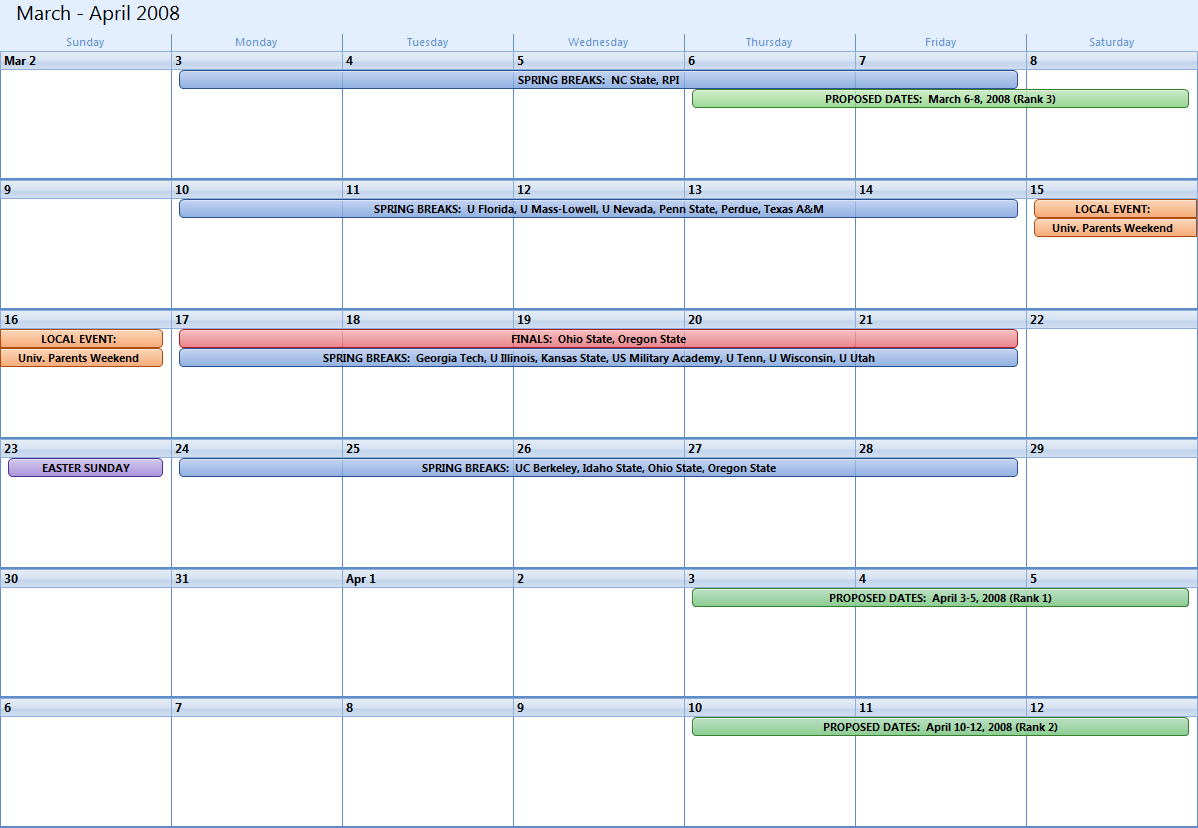
\includegraphics[width=16cm]{conference_dates.png}
\caption{Example calendar of ranked conference proposal dates.}
\label{fig:conference_dates}
\end{figure}

\subsubsection{Attendance Projection}
Planning requires an estimate of the number of students and professionals that are expected to attend the conference. Use numbers from previous conferences in attendance projections. Conference attendance figures, as well as the companies and universities which were represented, can be found in previous conference reports or programs (usually found on past conference websites). This can also be obtained by contacting past conference Chairs, SSC, and ANS National Staff.

Factors to consider the proximity of other student sections to the conference location, the number of students in each nuclear engineering (NE) department or program, and the number of students in the section's NE department/program. The size of each can be found on departmental websites or in the ANS bi-annual publication, \href{https://www.energy.gov/ne/downloads/nuclear-science-and-engineering-education-sourcebook}{Nuclear Engineering Education Sourcebook}.

\paragraph{In the Proposal:}
\begin{itemize}
    \item{State the number of students and professionals that are expected to attend and provide a justification for that number. If it is significantly smaller or larger than recent conferences, discuss why it is different.}
    \item{Describe contingency plans for if attendance is significantly higher or lower than the planning number. (Attendance cannot usually be reliably predicted until about one month before the conference.) \emph{Both scenarios can have significant implications on the conference expenses.}}
\end{itemize}

\subsubsection{Preliminary Program}
At the proposal stage, the preliminary program should consist of a detailed schedule of events (to the nearest quarter-hour) and corresponding descriptions of these events. It is important to lay out the activities of each day in order to demonstrate the flow of the conference, highlight potential event conflicts, and gain an idea of needed facilities. \textit{\textbf{Events competing with student research presentations should be minimized as they will cause you endless headaches.}}

The bare minimum for a student conference is: a welcome event/registration, student research presentations, a career and university fair, one SSC meeting, and an awards presentation. This minimum would make a boring conference. Additional events (prominent speakers, meals, a social, local tours) are highly encouraged, but the specifics of those events are up to the proposal committee.

It is expected that the schedule will continue to evolve as the planning process progresses. For example, tours may only be available on a certain day, or a local event may impact the initial plan. Additional groups, such as the host institution, sponsors, the SSC, or other ANS groups may request time and space to host events, at the discretion of the hosts (discussed in further detail in the Planning Manual). However, the schedule of events in the proposal should be complete enough for judges to gain an idea of the proposed ``attendee experience” and to assess the level of detail, foresight, and flexibility that has been put into the planning.

\paragraph{In the Proposal:}
\begin{itemize}
    \item{Include a graphical schedule similar to that shown in Figure \ref{fig:example_graphical_schedule}.}

    \item{Include a write-up which discusses each event.
    \begin{itemize}
        \item{Present potential event logistics, such as catering, audiovisual services, room setup, and travel (to offsite events).}
        \item{For non-standard events such as workshops or industry interaction, discuss the benefit/value of events to the participants.}
        \item{This is a great place to demonstrate leadership and vision by highlighting improvement and innovation over past conferences.}
    \end{itemize}}
\end{itemize}

Keep in mind the following suggestions. Student research presentations are traditionally 20 minutes (15 to present and 5
for questions). Be realistic about \textit{hidden time}: downtime between events, time to travel between facilities, time required to convert a room from one setup to another, time required to set up catering, and time required to clean up a room after each event. \textbf{Remember the focus of the conference: professional development and employment of students.} The time spent on various activities should reflect this focus.

\begin{figure}[h]
\centering
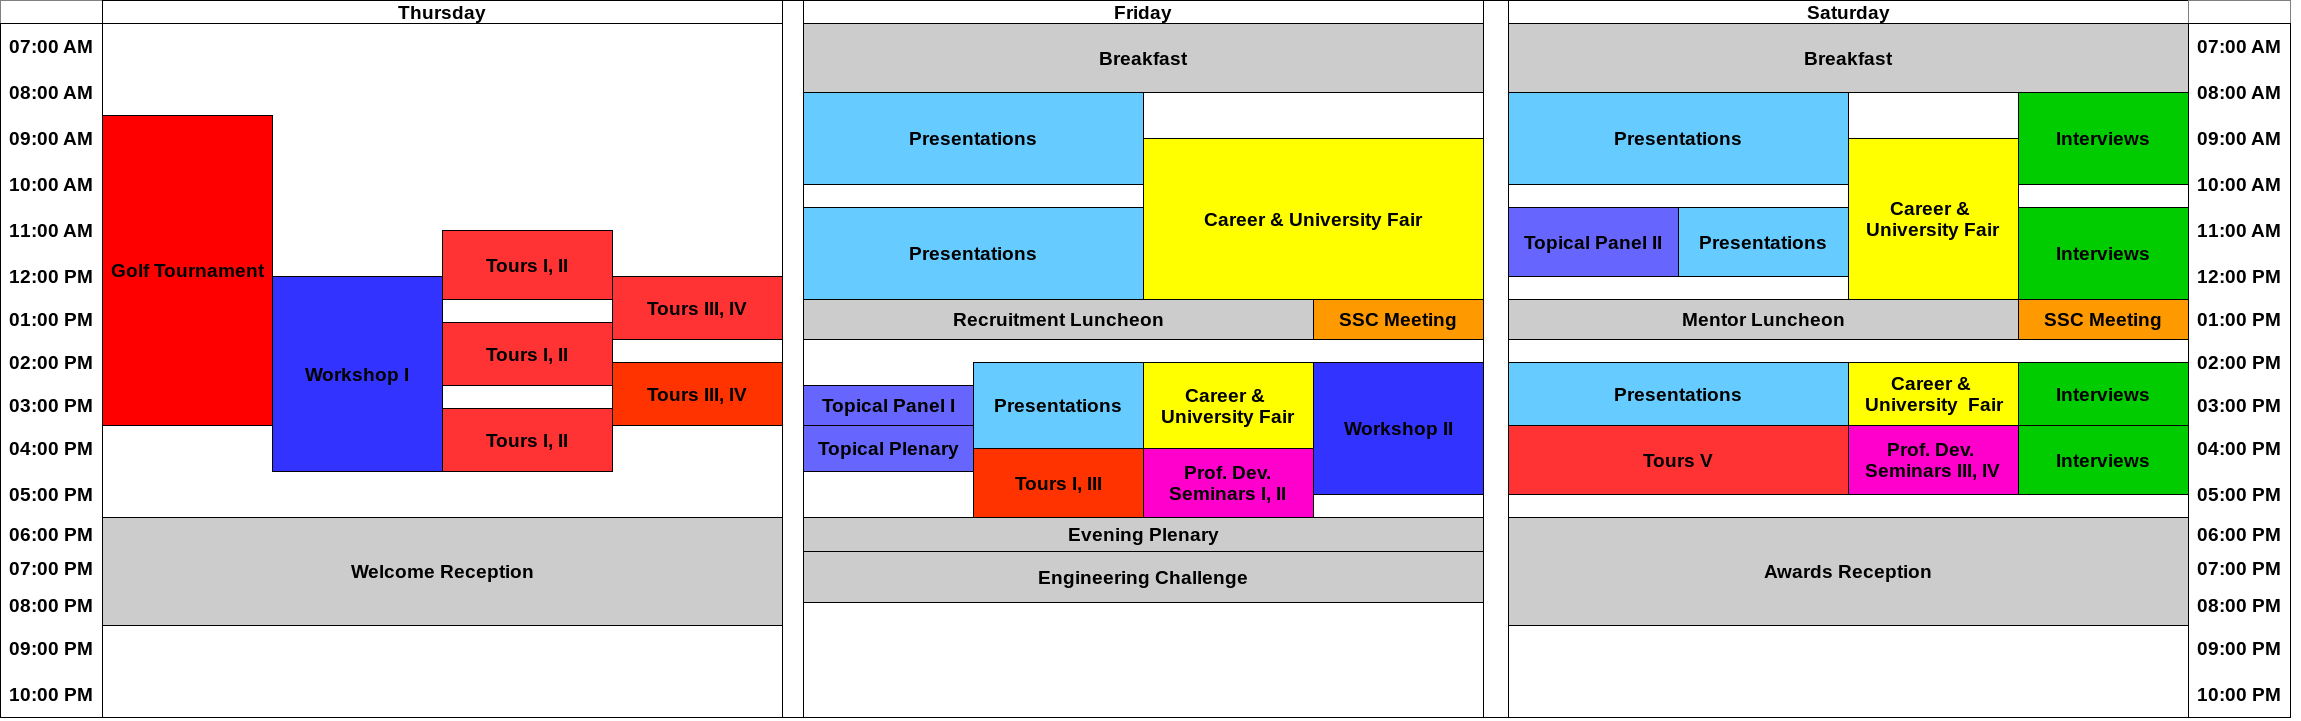
\includegraphics[width=17cm, height=7cm]{example_schedule.png}
\caption{Example graphical schedule of conference events/times.}
\label{fig:example_graphical_schedule}
\end{figure}

\subsubsection{Facilities}\label{sec:conference_facilities}

Getting adequate conference facilities for the desired dates is a crucial part of planning the conference. The conference cannot be hosted without adequate facilities. Conference facilities which are large enough to host the Student Conference are hard to find and are usually booked solid far in advance. Creative compromises between dates, events, and facilities should be expected.

\textbf{Do not place any sort of deposit down to reserve these facilities, leave this to ANS National. Likewise, do not personally, or on behalf of the student section, enter into any contracts related to the conference. This is to protect the proposal committee from any liability that they may incur from not fully meeting the terms of the contract, especially if the proposal is not selected. ANS National is not responsible or liable for any contracts that they have not signed.}

Past conference hosts have sometimes found that their preferred facilities were booked by someone else in the time between the proposal submission and the announcement of the conference host. If the preferred facility does not require a deposit or official contract, consider reserving it for the preferred date even before the proposal is submitted. Otherwise, request a soft hold from the facility manager for those dates with instructions to inform you immediately should they become contested (right of first refusal).

\paragraph{In the Proposal}
Use the provided forms on the SSC website to:
\begin{itemize}
    \item{Identify and describe the prospective conference facilities and amenities.}
    \item{Estimate the number, type, and size of rooms required based on the preliminary program.}
    \item{Give a detailed schedule for each room based on the preliminary program. Include room capacity, projected attendance, desired room setups, catering, and audiovisual requirements for each event. Include setup and takedown time.}
    \item{Include a graphical room schedule similar to that shown in Figure \ref{fig:example_room_schedule_1}.}
\end{itemize}

\begin{figure}[h]
\centering
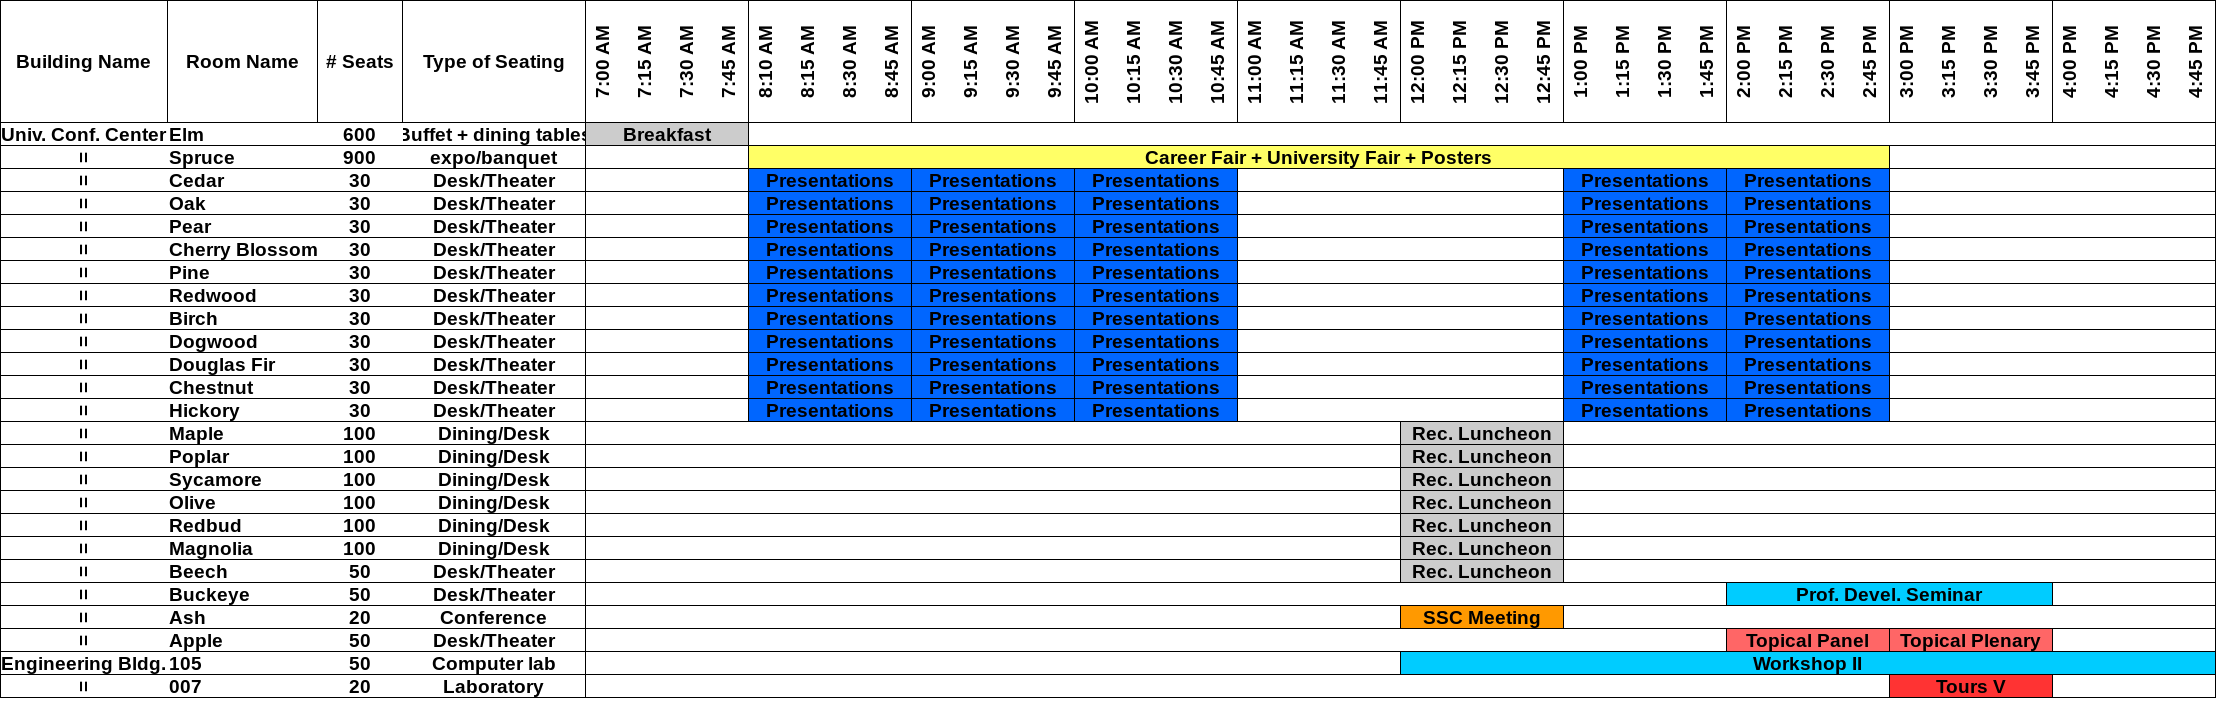
\includegraphics[width=18cm, height=6cm]{example_room_schedule.png}
\caption{Example room schedule, graphical version.}
\label{fig:example_room_schedule_1}
\end{figure}

\clearpage

%\begin{figure}[h]
%\centering
%\includegraphics[width=16cm]{example_room_schedule_2.png}
%\caption{Zoomed-in version of the example room schedule.}
%\label{fig:example_room_schedule_2}
%\end{figure}

\subsubsection{Hotels}
Choosing hotels can be challenging because you are constrained by costs, proximity to the conference, and proximity to each other. Clustered hotels make for better transportation logistics. It is very important to account for unexpected delays when scheduling transportation from conference facilities to hotel accommodations such as traffic, loading and unloading time.

A best practice is to involve the ANS Conference Staff in the hotel negotiation process after your bid has been accepted. They have experience negotiating with hotels and can help you get the best deal, and giving information to the hotels before they are involved can reduce their ability to negotiate. The hotel contract should be signed by ANS National, not the student section.

The size of the hotel room block (which will not be the maximum capacity of the hotel itself) should be consistent with attendance projections. It is reasonable to assume that students will book 4 per room and professionals will each book their own room. Also, consider that some professionals will only stay one or two nights of the conference. Depending on the availability, the conference facility may be sufficient to host the entire room block, or more than one hotel may be required. Like conference facilities, hotel reservations may be booked 18 months or more in advance by outside groups and may impact the conference dates, so discussions with hotels should begin early.

As with other aspects of the proposal, keeping the cost to students at a minimum is important. When making travel plans, student sections will typically look for the cheapest hotel options available, even if it is not at the official conference hotel. If room rates are prohibitively high, consider creative arrangements, such as subsidizing student rooms by paying a flat fee to the hotel.

Identifying multiple options for hotels in the proposal is strongly encouraged. However, reserving too large a room block can be as just as bad as, if not worse than, reserving too small a block. If a large number of rooms that are reserved in the room block go unused, the hotel may charge the conference for each of these rooms and nights to make up for lost revenue, known as attrition. Consider policies that encourage students to stay at the conference hotels, rather than the cheapest option available, to reduce the risk of attrition. This concern is more significant for the conference planning process, but should motivate proposals to be as accurate as possible with attendance and hotel predictions.

\paragraph{In the Proposal:}
\begin{itemize}
    \item{Identify the first and second choice sets of hotels as well as capacities. Minimize any discussions with hotels that do not include ANS Conference Staff.
    \begin{itemize}
        \item{Give the base price you can find online or without entering into detailed discussions with the hotel.}
        \item{Provide the maximum number of hotel rooms the hotel is willing to block out.}
    \end{itemize}}
    \item{Include a map which shows the proximity of hotels to conference facilities.}
\end{itemize}

\subsubsection{Transportation}

The proposal should address transportation to, from, and during the conference.

\textbf{To/From:} The cost of air travel for the different student sections to the conference city needs to be estimated in order to determine travel assistance costs for the budget. A means of transportation from the conference airport(s) to the conference hotels must also be identified. These can be airport shuttles, conference provided shuttles, public transit such as a metro, or (as a last resort) hotel provided shuttles.

Don't forget to take into account the capabilities of the planned airport destination(s), as well as the capacities of the various transportation services available. For instance, if the local airport is not capable of handling the traffic, or is so small as to be noticeably more costly, list alternatives as well as plans to accommodate those alternatives. Consider what parking options are available at or near the conference hotels for attendees who are driving (pay parking is acceptable).

Do not assume that the reviewers (or attendees) are familiar with transportation options; if there's a hole in the proposal plans, it will likely be noticed! Historical airfare prices for various city pairings and times of year can be found on several major travel reservation websites.

\textbf{During:} Shuttle transportation for students from conference hotels to the conference site(s) and between conference events at different sites should be provided if the distance is further than 1/3 mile. Professionals may choose to take the shuttle or take their own transportation to the conference site(s). As with the hotels, adequate parking at the conference facilities for those who choose to drive. A 40 minute round trip time from hotels to the conference site should be considered an upper limit. Remember to account for loading/unloading of passengers.

\paragraph{In the Proposal:}
\begin{itemize}
    \item{Air Transportation
    \begin{itemize}
        \item{Identify local airports.}
        \item{Estimate air travel costs per attendee for representative Student Sections.
        Estimates should correspond to the first choice conference dates.}
    \end{itemize}
    }
    \item{Ground Transportation
    \begin{itemize}
        \item{Identify how students will get from the airport to their hotels.}
        \item{Include the trip length from a local airport, and suggest a departure frequency.}
        \item{Identify how students will get from their hotels to conference events and between conference events.}
        \item{Include the trip length, and suggest a departure frequency.}
    \end{itemize}
}
\end{itemize}

\subsubsection{Budget}
Ideally, the budget should predict the cost of the conference (and thus the fundraising requirements) within 5\%. The judges examine the detail, accuracy, and thoroughness of the budget. Past conference proposals have tried to make their conference appear as economic as possible by low-balling or omitting numbers. While a low total budget number may impress the judges, the judges will be more impressed by a complete budget that considers all expected costs. Be forward and honest about financial figures: the actual numbers will not help or hurt the proposal, assuming they are reasonable.

The budget will continue to evolve as planning and fundraising progress. Guidance on final budgets and the budget process can be found in the Student Conference Planning Manual on the SSC website. Here are a few things to consider when drafting the proposal budgets:

\begin{itemize}
\item{A student travel assistance package should be included as a planned expense in the budget (that is, money towards travel expenses for those coming from out-of-town to the conference). A good target is to give back 100\% of student travel expenses. It is reasonable not to include expenses such as food, lodging, and registration fees.} The proposal budget will likely benefit from researching past student conference travel assistance amounts.
\item{Revenue (fundraising) targets in the proposal should be 10\%-15\% higher than expected expenses, including travel assistance.}
\item{ANS National provides \$5,000 in seed money and expects to get this money back (it is an interest-free loan, not a gift)}. They also take a 25\% cut of the profits (calculated after travel assistance); this 25\% goes towards covering services provided by ANS, such as administrative support, personnel time, and other necessities.
\item{If the conference's fundraising efforts result in greater revenue than projected, the organizers will be expected to increase student travel assistance amounts, the contributions back to ANS, and direct contributions to next year’s conference in order to keep their profits at a reasonable percentage. If the fundraising is lower than targeted, the first thing to be cut is the host section’s take of the profits.}
\end{itemize}

\paragraph{In the Proposal:}
\begin{itemize}
\item{Include a detailed, realistic, and complete budget. The budget should correspond to the dates, projected attendance, preliminary program, facilities, and transportation in the rest of the proposal.}
\item{Divide the budget into two sections: (1) expenses and (2) revenue. The expenses section should be further divided into two subsections:
\begin{itemize}
\item{\textbf{operational expenses} are the essentials required to host the conference (e.g. food, facilities, mobile app, and travel assistance).}
\item{\textbf{discretionary expenses} are the non-essentials (e.g. socials, attendee gifts, awards) and can be cut if there are revenue shortfalls.}
\end{itemize}
}
\item{Discuss a fundraising plan to raise the necessary revenue. The plan should be realistic (\$ per contributor) and achievable.}
\item{Identify the order of budget cuts should fundraising not succeed. It is strongly emphasized that travel assistance \textit{is the last thing to be cut} and that this may mean reduced socials or that the host section takes no profit.}
\item{Include the following figures of merit that summarize the budget:
\begin{itemize}
\item{total target revenue}
\item{total expenses, subtotaled by operations expenses and discretionary expenses}
\item{cost-per-student (total conference expenses divided by total number of expected student attendees)}
\item{cost-to-student (average estimated out-of-pocket costs for each student attendee that does not attend the host university, not including travel assistance)}
\item{average planned travel assistance per student}
\end{itemize}
}
\end{itemize}

Revenue sources include registration fees, career fair exhibitor fees, sponsorships, and donations. Fundraising for previous conferences can be estimated by tallying the sponsors listings in past conference programs. However, more reliable numbers may be found by asking past conference Chairs. The ANS professional divisions historically have made significant annual donations to past student conferences, but (under the One-ANS change in 2019) have less ability to do so and should not be relied upon.

A word of caution about registration fees: the final registration revenue needs to account for complementary registrations that are provided to VIP's or sponsors. Again, reliable figures can be found by talking with past conference hosts and ANS National.

\subsubsection{Banking and Financial Oversight}
Conference hosts should have a system for handling checks, cash, credit cards, and taxes. Where possible, conference money should be separated from other section transactions. Additionally, an oversight mechanism should exist for all transactions (for example, a bank account where every financial transaction requires the signature of two officers).

The tax-exempt status of a student section and the student conference is not to be assumed! Some sections never achieved tax-exempt status, or had tax-exempt status but lost it by failing to file appropriate IRS forms. Some sections are tax-exempt because of their affiliation with their student union or host university. Some sections independently filed for tax-exempt status with the U.S. Internal Revenue Service (IRS). Every section’s situation is unique, but \textit{not all past conferences have achieved tax exempt status.} ANS National is not tax-exempt everywhere!

\textbf{It is illegal for ANS National to transfer funds to to secondary tax-exempt accounts, do not suggest this.}

ANS National can provide banking services to the conference and we \textit{strongly encourage} you to use this as your first option. This is the preferred system as it allows easy oversight and they have experience managing large conference donations. Some student groups may have university regulations that do not allow this system. Secondary accounts, such as those maintained by the host university or the student section are also allowable, your bid should detail how you went about identifying if this applies to your bid.

Many schools have a student organization bank which is already set up to provide sufficient financial oversight over student section accounts. Credit, debit, check, or ACH can be used when no better options are available.

\paragraph{In the Proposal:}
\begin{itemize}
\item{Identify the banking system to be used by the conference.}
\item{Identify the financial oversight mechanism for conference banking.}
\item{Identify options to achieve tax-exempt status.}
\end{itemize}

\subsubsection{Conference Committee Organization}

The organization of the conference committee should be customized to the strengths and
weaknesses of its members. Many organizational structures have worked successfully in the past. Whatever is chosen, responsibilities and reporting structure should be clear. The decision-making process of the committee should also be established. Typically the conference Chair(s) have full authority over the conference committee and ultimate responsibility for the success of the conference. However, there should be a formal set of written conflict resolution procedures for the committee, developed before any conflict occurs.

\textbf{Conference Chairs} The decision on who will be named as Conference Chair(s) is a very important one, as these persons will likely be the face of the conference.
The students selected as Conference Chairs should have previous experience and participation in national ANS conferences.
Certain responsibilities must also rest closely with the relevant Chair. All of the highest-level responsibilities will likely fall to the Chairs in the end; budget management, fundraising, interfacing with important speakers, and overall logistical coordination are Chair-level responsibilities. These responsibilities should not be assigned to a lower-level committee member.

\textbf{It is common that a Student Section’s first proposal is not selected, and the proposal is re-submitted in a later year. This often means the graduation of the students behind the original proposal effort and a change in the named conference Chair(s).} The visionary leadership and organization skills of a Chair who authors a proposal can be evaluated through the quality of that proposal. Unfortunately, a successor Chair can inherit the proposal. Because of this, if a named Chair changes between proposal submissions without substantial changes to the proposal, additional detail about the new Chair is required in the proposal. If a named Chair changes between awarding of the conference and the conference dates, a similar process will need to be followed. In rare cases, if the SSC does not feel a replacement Chair is suitable, they may direct the selection of a new Chair or even change the conference to the runner-up school.

\textbf{Conference Committee} Committee members also play an important role in managing the day-to-day affairs of the conference. The proposal will need to detail not only what these available positions will be named, but also what their duties will be, as well as perhaps a preliminary naming of who would fill these roles. During the planning process, additional responsibilities may arise. This structure can act as a guideline in assigning tasks to the various committee members. It is also common for the conference committee members identified in the proposal to change, even if the proposal is selected after its first submission. Identifying backup committee members or understudies may be helpful to the proposal. Proposal committees are encouraged to examine successful proposals from past years to see more specific examples of organizational structures and positions.

\paragraph{In the Proposal:}
\begin{itemize}
\item{\textbf{Organizational Chart:} Provide a graphical organization chart showing titles.
Identify a person to fill each position.}
\item{\textbf{General Areas of Responsibility:} List the general responsibilities of each
position.}
\item{\textbf{Past Experience:} Include a listing of past student and national ANS conferences
each committee member has attended. Participation in other professional
organizations may also be mentioned. The conference Chair(s) are generally expected to attend at least one student conference and one professional conference before submitting a proposal.}
\item{\textbf{Letter of Endorsement for New Chair(s)}: If the named conference Chair(s)
have changed since a previous proposal submission but the proposal has not
substantially changed, then include a letter of endorsement of the new Chair(s).
\begin{itemize}
\item{consists of at least 400 words but less than two pages}
\item{presents the reason the specific individual(s) were selected as the new Chairs(s).}
\item{addresses the vision, leadership skills, and organizational capabilities of the
individual(s), preferably with examples or past experience}
\item{is authored by someone personally familiar with the Chair selection process}
\item{includes as many signatories as deemed necessary to be persuasive}
\end{itemize}
}
\item{\textbf{Decision Making Process:} Draft a set of procedures or operating guidelines for the conference committee.
\begin{itemize}
\item{Identify the procedure for removal/addition/replacement of a committee member, especially the committee Chair(s).}
\item{Define the Faculty Advisor’s authority.}
\item{Identify what kinds of decisions can be made by which conference committee members (e.g., decisions that require spending money).}
\end{itemize}
}
\end{itemize}

NOTE: It is highly encouraged that Technical Chairs (or whoever is in charge of the technical program) be someone who has experience at technical conferences, as this role will involve coordination and handling of submission/review process. This experience is usually carried by a graduate student.

\subsubsection{Schedule/Milestones}
As with any large project, there are many sequences of tasks which must be completed in parallel. Tasks are interrelated and the judges need to see that you have identified which tasks you need to accomplish and generally the things that depend on them.

One method of balancing these sequences is with the use of milestones: tasks that represent the endpoint or convergence of several task sequences at once. A good example of a milestone is the opening of registration. In order for registration to open, the website must be operational, the conference starting and ending times must be known, and all information needed from participants for the various events must be identified (e.g., meal choice, flight info and hotel info for transportation, software user license information for workshops).

The proposal should present this schedule in a clear and logical fashion so that judges can assess if there are any missed items or potential problem areas. Project planning tools (e.g. Gantt charts) may be helpful.

\paragraph{In the Proposal:}
\begin{itemize}
\item{Identify major milestones and provide target dates for their completion. For each milestone, identify key tasks that must be complete to meet the milestone.}
\item{Identify other critical tasks that must be accomplished (not necessarily tied to a milestone).}
\item{For each key or critical task, identify who is responsible for it, when it should be completed by, and if there are any predecessor tasks that must be completed first.}
\end{itemize}

\subsubsection{Staffing}
The hosting student section must have enough active students to support the conference effort. Having 10 dedicated students serving as the primary organizers for the conference, with an additional 20 students to staff the events, is recommended given the size of recent conferences. If the hosting section or department has fewer than 30 members, it may be necessary to recruit outside volunteers to help organize and staff the conference.

Arrangements with other groups (such as other departments or student societies) for additional staff should be presented in the proposal. Another possibility for staffing the conference is to make arrangements with other ANS student sections. For example, staff assisting with technical sessions could  be from another section. The larger and/or geographically closer sections will likely be able to provide the most volunteers. A section could volunteer their services free-of-charge or in exchange for some compensation such as guaranteed travel assistance or registration discounts. \textbf{There is no reason to be short-handed on volunteer staff during the conference.}

\paragraph{In the Proposal:}
\begin{itemize}
\item{Identify the number of day-of staff needed to execute the conference and describe how this number was obtained. Keep in mind that this will change, but use it as a starting point for engaging students at your school.}
\item{Describe the roles of each group of day-of staff and state which conference committee member each staff group will report to.}
\end{itemize}

\subsubsection{Liability}\label{sec:liability}
ANS and the conference hosts inevitably assume some liability (risk). The common areas of liability are finances, contracts, and negligence. \textbf{You must consult ANS National about any contracts or liability issues. As a reminder, ANS National is not liable for any contracts that they have not signed.} Examples of liability that might be encountered during an ANS Student Conference include:

\begin{itemize}
\item{Any contracts that define a payment schedule and a financial penalty if the schedule is not met.}
\item{A hotel requires a certain number of rooms to be paid for, or else will asses a financial penalty (attrition).}
\item{A social event requires minimum purchase of food and drink.}
\item{Financial penalties for overdrawing a bank account.}
\item{Any event that serves alcohol (someone could drink too much and hurt themselves or someone else; someone could drink underage).}
\item{Damage to an attendee's or borrowed property during official conference events (e.g. a fuse blows and shorts out ten university laptops, the career fair room may be subject to theft).}
\item{Any event that could cause physical harm to an attendee. (Hint: all events could. Consider slips/trips/falls, food  poisoning, and vehicle accidents in addition to more exotic risks like a skydiving social and drowning during a riverboat cruise.)}
\item{The student section may owe federal or state taxes on student conference profits in certain situations.}
\item{Theft or accidental release of private information, especially that of private information associated with minors.}
\end{itemize}


\paragraph{In the Proposal:}
\begin{itemize}
\item{Identify known and potential liabilities.}
\item{For each, discuss whether that liability will be carried by the student section, the university, ANS National, or the host facility. Indicate whether the group has already agreed to carry this liability if this is the case.}
\item{Consider whether any of these activities will ultimately require waivers to be signed by the participants. \textbf{ANS National must be consulted for help in this matter.}}
\item{Discuss any additional steps that are being taken to minimize the risk (e.g. ANS National reviews contracts, drink tickets at the social, liability insurance policy).}
\end{itemize}

NOTE: Should the proposal be selected, all liability should be clearly understood and documented before the conference takes place. The SSC Chair and ANS National can help the planning committee through this process.

\subsubsection{Support}
Institutional support from the student section's department and college are important to being able to successfully host a conference.
It is strongly recommended to engage key administrative figures, such as the Department Head or Deans during the proposal process to discuss the needs of the conference and what the department or college can provide to the conference, if selected.
It is also beneficial to show local support behind a student section’s proposal.
If the section is small or has not been active in recent years, a show of student support is also
recommended.

\paragraph{In the Proposal:}
\begin{itemize}
\item Include a letter of support from the:
\begin{itemize}
\item{Student section Faculty Advisor}
\item{Department Head}
\end{itemize}
\item{Include contact information for relevant university hospitality/facilities/events staff. We encourage you to involve them in this process if your bid is accepted.}
\end{itemize}

\paragraph{For Bonus Credit:}
\begin{itemize}
\item{Include a letter of support from the:
\begin{itemize}
\item{ANS local section}
\item{Engineering school Dean}
\item{Students in the student section (particularly recommended for smaller sections)}
\end{itemize}
}
\end{itemize}

NOTE: Letters of support from anyone outside of ANS or the host university (for example,
potential corporate donors) will not be considered. If these are added to the
proposal anyway, these pages will be removed from the proposal before it is given to
the judging committee and the proposal will be penalized. See Section \ref{sec:special_cautions}.

\subsection{Leadership and Vision} \label{sec:LandV2}
The conference organizers demonstrate leadership and vision by having a clear idea of
what their conference will be like, both mechanically from the logistics side and
aesthetically from the participant’s side. The leadership and vision component of the
proposal is made up of less tangible elements that are harder to quantify. These elements
are subjectively rated by each judge, usually on a weighted or sliding scale. This section
of the document outlines some general concepts and ideas that the judges may look for.


\subsubsection{Theme}
The Student Conference traditionally has a theme, chosen by the organizers and indicated
by the title of the conference. The theme should be clear---it's meaning should be obvious---and should ideally focus attendees on an aspect of nuclear science and
engineering that they might not otherwise spend much effort on. Past examples include:
\begin{itemize}
    \item “Expanding the Nuclear Family” (Texas A\&M, 2008),
    \item “Nuclear Science and Technology: Past, Present and Future” (University of Nevada, Las Vegas, 2012)
    \item “Being a Critical Member of the Nuclear Industry” (University of Wisconsin-Madison, 2016),
    \item "Saving the World One Atom at a Time" (University of Illinois Urbana-Champaign, 2022),
    \item "Passing the Torch" (University of Tennessee Knoxville, 2023),
    \item "Keystone of Tomorrow" (Pennsylvania State University, 2024),
    \item "Old and Nu" (University of New Mexico, 2025),
\end{itemize}


The theme should be central to the conference, rather than tacked on. In the proposal, the theme can be best reflected in the discussion of the planned events. Speakers can
be invited to address specific topics. Workshops can be focused on areas related to the
theme. Material provided to participants can elaborate on the theme. A good theme will be apparent during the conference proposal and planning by the way it shapes the conference.

\subsubsection{Participant Experience: Event Design}
Each event should be carefully thought through from beginning to end, but the judges do not want to see that you have done all of the thinking already (we want to see ideas and your plan for deciding things). Events will change, details will change, we want to see that you have options, theme ideas, and suggestions for what you will do. Ask yourself: how does it enhance the conference?; how does it alter the participant experience?; and how does it meet the goals of professional development and employment of students?

It is pretty easy to recall events you liked, events you didn’t, what you liked about them, and what you thought could have been done differently. Events should always be crafted with their intended benefit(s) in mind. Adding features or aspects to an event that do not support the intended benefit will merely make the events confusing, difficult, and expensive. Expect for new and improved events to be evaluated by the judges based on the perceived value/benefit to the participants. (Not all events require a lofty goal; benefits may be as simple as “attendees have fun”.)

EXAMPLE: You believe that students at the conference should be able to do more than just meet career fair booth exhibitors; they should also be able to accelerate the hiring process. In response, you provide recruiters with interviewing facilities and allow them to schedule students to interview on the spot.

EXAMPLE: You feel that students need help networking because many are adorably awkward in those pre-graduate years. In response, you design a mentor luncheon where students are seated with professionals in their field of interest by table.

\paragraph{A Special Note Regarding Socials}
Socials should be considered extra-budgetary and not divert funds away from professional activities or take precedence over student travel assistance. Liability regarding socials should be thoroughly addressed (see Section \ref{sec:liability} regarding liability).

Socials should only support a conference and never take away from it. The judges will assume that people will take part in every event possible. Based on this, socials (and any other events) should allow participants adequate breaks and a minimum of 8 hours sleep per night. For example, do not have a social that is scheduled to run past 10 pm unless it is the last night of the conference. Pay particular attention to Thursday and Friday evening events that might be physically strenuous or involve alcohol---these could deter participants from attending technical sessions.

\subsubsection{Participant Experience: Details}
The proposal should not need to have every detail of every event planned! Prices, locations, vendors, contacts, etc. two years in advance will always change and you will not impress the judges by providing everything. You will impress the judges by giving context (maybe there's a pricing plan available on an event space's website, maybe you can give context on pricing for your school community).

As with event design, we want to see that you appreciate the attendees’ perspective and have thought about it. Ideally the events will leave the largest impression, but great event design can be completely overshadowed by logistical details. Your proposal should demonstrate the level of detail that the committee is working at so the judges can assess their ability to handle the small things. That being said, the big-ticket items will likely be most closely scrutinized---number of attendees, length of time for events and the conference itself, availability of transportation, etc. are all things that could play a critical role in whether the reviewers feel the student section is ready to host the student conference.

When planning conference logistics, look to build on and improve upon past conference events. Think again about past student conferences, national meetings, topical meetings, meetings of other societies, events held by community groups, and any other large-attendee event you have attended. Instead of focusing on the main event, consider the surrounding details: facilities, furnishings, audiovisual equipment, timing, transportation, ease of finding information ahead of time. What worked well? What would you change?

EXAMPLE: You found it hard to enjoy a plenary because you were more concerned about when dinner was going to be served. So in your proposal you mention you will have event details for dinner events with the order of events.

EXAMPLE: You never knew how long a shuttle trip from the hotel to the conference site would take or how long you would have to wait for the bus. This made it hard to plan your first day. So in your proposal you mention that bus schedules will be included in the conference app and posted on the conference website.

\subsubsection{Proposal Attributes}
There are several qualities of a good proposal that typically influence the judges in some way. The following are words that judges often use when discussing proposals (and are also listed on the \emph{Judges' Evaluation Worksheet}). These qualities should be apparent in both the proposal document and the conference vision.

\textbf{Organization}---The proposal should flow in a clear and logical fashion.

\textbf{Clarity}---The judges should not have to work hard to figure out what the proposal is trying to say.

\textbf{Professionalism}---A good rule of thumb when designing the conference is: “professional conference first and student conference second.”

\textbf{Originality}---Every student conference is different and every university has something unique to offer. Highlight it.

\textbf{Comprehensiveness}---If it’s not in the proposal, judges often assume it has not been considered (show us how you will decide things, not that you have decided them). This should not be at the expense of conciseness.

\textbf{Responsibility and Integrity}---Conference hosts must uphold the reputation of the ANS and the host university. Be transparent in financial dealings, avoid conflicts of interest, and properly prioritize (student travel assistance before profit, student interests before corporate
interests, professional development before socials).

\textbf{Productiveness}---The conference should tend to the professional, academic, and employment needs of the participants.

\textbf{Fun}---The conference should be interesting and enjoyable for participants. Avoid boring events, dull speakers, and sessions of extended length.

\textbf{Aesthetics and Image}---How visually appealing is the proposal? How is the theme represented? This is a chance to show off branding, design, and marketing skills. These will be particularly important for fundraising.

\textbf{Economy}---The costs to students must be reasonable, as must the fundraising expectations. Does the proposal have a contingency plan for cutting costs, if needed? Could a similar experience be obtained for cheaper?

\textbf{Overall Proposal Quality}---The quality of the proposal document implies the quality of the eventual conference. The skills necessary to write a good proposal are the same ones needed to write a good fundraising letter or speak to gathered attendees. Grammar and spelling count.

\subsubsection{Student Section Strength}
In the year leading up to the proposal, the applying student section needs to demonstrate its strength, both at the local and national level. The proposal should summarize the strength of the student section, citing examples for the benefit of those judges who may not have personal knowledge of the section.

Activity at the local level is gauged by indicators such as the size of the section, attendance at its events, the complexity or budget of its regular yearly activities, and its involvement and collaboration with the local section.
Activity at the national level is typically measured by national/student conference attendance and Student Sections Committee (SSC) participation. National conference attendance implies student section strength and resources.
Student conference attendance implies the student section fully appreciates the scope of the task of hosting a student conference.
SSC meetings are held at every national and student conference and attendance by a representative of each section is expected.
\textit{Participation at SSC meetings by Section representatives and the
proposal committee is the best-correlated predictor of who wins the conference.}

\subsection{Proposal Presentation}
At the end of the day, the proposal document should be the student section's best document; whatever is submitted should be representative of the best abilities of the section. However, there are a few guidelines to follow when writing the proposal:
\begin{itemize}
\item{\textbf{Conciseness}---Unnecessary ``fluff” or 10 pages describing the school history or meal options copied directly off a website do not add value to the proposal. On the contrary, a proposal that is not to-the-point simply wastes the judges’ time and patience. Remember that the judges
are real people, so talk to them, through the proposal, like they are real people.}

\item{\textbf{Summarization}---Consider including an Executive Summary (a one page section of the proposal that comes
between the title page and the table of contents). The executive summary should hit all
the high points of the proposal committee's conference vision and focus on facts, not opinions.}

\item{\textbf{Support}---All supporting documentation, such as letters from a department head, should appear in appendices. All worksheets and calculations should be placed in appendices. Only worksheet summaries or calculation results should appear in the body. Tables and illustrations should be used whenever they result in greater clarity and conciseness.}
\end{itemize}

\subsubsection{Writing Software}
There are a variety of options to use for drafting the report.
A few (most certainly not all) of the choices available are:

\textbf{\LaTeX}\newline
A very well-known typesetting system for drafting papers and reports, LaTeX has the advantage of easy manipulation of typesetting, broad community support (helped by being completely open-source), and portability---a document's source code can be edited by any text editor and will give near-identical or identical results across a wide range of systems. In addition, there are many online platforms, including Overleaf and Authorea, that allow multiple users to collaborate on one document, meaning no single person is given the dubious honor of compiling multiple conference documents into one cohesive whole. One disadvantage is that those new to LaTeX (or any typesetting language) will need to learn how to use it; however the learning curve is not very steep and is significantly reduced if one is already familiar with programming.

\textbf{Adobe InDesign}\newline
There also exist several professional products capable of drafting a proposal document, such as Adobe InDesign, used for producing flyers, brochures and other visual media. The advantage of software such as this is that---unlike Latex---it is built with the express purpose of creating things like conference proposals, and thus possesses a variety of professional tools useful for pulling together a document more rapidly than an equivalent Latex document. Since it is used in industry this also means that by default it possesses some features which would be harder or even impossible to achieve in other document preparation software without going to unreasonable lengths.

\textbf{Word Processors}\newline
Many people are familiar with word processors such as Microsoft Word or OpenOffice Writer, and thus, preparing a document with this format is considered relatively straightforward. However, it can be difficult to prepare a large document in this manner, and fine control can often be an issue when compared to other software packages. In addition, a document prepared on one machine might have issues when brought over to another machine with a different version or a different operating system.
Another alternative is using Google Documents, which another word processor, but is operating system-independent, allows for multiple users to edit online, and offers built-in version control.

\newpage
\section{Submission}
Sections interested in submitting a proposal should inform the SSC Chair of their intent to submit a proposal, so that they can receive important updates as necessary.
Submissions are due roughly \textbf{18 months} in advance (typically around October 1st).
The exact date will posted to the \href{http://students.ans.org/THELINK}{SSC website} around mid-April
An announcement will also go out to all student section presidents (provided the current officer information is on file).

Proposals should be emailed to the (\href{mailto:sscChair@gmail.com}{SSC chair}).
All proposals \textbf{must be submitted in PDF format} and are limited to 10 MB in size.
Alternatively, the applicants may host the proposal on a web server and notify the SSC of the URL by the deadline date, although this does not eliminate the 10 MB size limit.
Hosts will then be chosen and notified during the President's Special Session during ANS Winter Meeting (typically early November).

\newpage
\section{Evaluation} \label{sec:Eval}
The proposal evaluation process is continuously evolving. The SSC’s expectations of the proposals change with each passing conference. To reflect these changing expectations, the \textit{Judges’ Evaluation Worksheet} is updated frequently by the SSC and the current \textit{Student Conference Proposal Guidelines} document is updated when necessary.
These regular changes reflect the increasing challenges of hosting the conference, responsibility of the conference hosts, the liability to the ANS, and the oversight obligation of the SSC.

Should any part of the evaluation process or this document be unclear, contact the \href{mailto:sscChair@gmail.com}{SSC Chair} for clarification.

\subsection{Evaluation Process}
Before the submission deadline, a judging committee is formed from members of the
Student Sections Committee (SSC). After the submission deadline, the submitted
proposals are distributed to all the judging committee members. The Judges’ Evaluation
Worksheet (discussed in the next section) and any additional guidelines, instructions, and supporting data are also given to the judges. The judging committee members read the proposals, deliberate and discuss them for approximately two to three weeks before
taking a vote.

During the deliberation and the discussion period, the judging committee members gather additional information that can help them in judging from a variety of sources.
Judging committee members may ask questions of the proposal authors via email, telephone, or personal meeting.
They may contact the SSC Chair to obtain information on past operations of the student section (annual report, outreach events, copy of Glasstone application). They may use the internet or call vendors or facilities to check information given in the proposal document. Judging committee members have also been known to contact alumni from the student section to ask questions about the strength of the section or to get an independent take on proposal items.

The judging committee’s decision for the next year's student conference is traditionally announced during a special session at that year's ANS Winter Meeting.
However, the timing of this announcement is subject to change. For instance, if the student conference falls unusually late in the semester or the winning school has identified a particularly early desired date for their conference, then the announcement might be rescheduled accordingly.

After the decision is announced, the judging committee provides written feedback to all submitted proposal authors.
This feedback will generally include mention of the judging committee’s perceived pros and cons of each proposal and suggestions for improvements
before resubmission the following year.
The judging committee will also provide
detailed guidance to the selected section about specific aspects of their proposal that should be addressed or considered when planning the conference.
The Winter Meeting is also an excellent opportunity to hear feedback or discuss in person how the proposal that were not selected could be improved upon.
This could prove instrumental in helping the proposal's chances the following year.

\subsection{Additional Criteria}
There are additional elements, not part of the proposal, that have frequently entered into the judges’ discussion in previous years.
None of the following are hard and fast rules.
Should there be concerns about the possible effect of any of these items on the chances for hosting, discuss them with the \href{mailto:sscChair@gmail.com}{SSC Chair} before pursuing a proposal.

\begin{enumerate}
\item{Strength and leadership of conference chairs is a key part of the judges’ decision.
A superior proposal is meaningless if the chairs do not have the ability to realize
it. The proposal document is assumed to reflect the leadership of the chairs.
However, the judges’ personal knowledge of the chairs (or lack thereof) may also
be a factor. Further, past ANS and non-ANS leadership roles and successes are
considered, especially with regard to student section activity.}
\item{Student Sections should be in “good standing”. Check the \href{http://students.ans.org/section-standing/}{SSC website} to
determine the section’s status. ``In flux” or ``inactive" standing can be quickly remedied, but it is best to accomplish this \emph{well in advance} of the proposal deadline.
(Sections which are not in good standing for many years prior to application, only to
miraculously file annual reports and submit draft rules the week before the
proposal deadline, are generally considered to have barely met this criteria.)}
\item{Similarly, the overall activity of the section is normally among the evaluation
criteria. While the section self-reports its strength and participation in the proposal, this is always compared to the record that ANS National has of the section’s activities. It’s important for sections to file \href{http://students.ans.org/outreach/}{outreach reports} and \href{http://students.ans.org/section-standing/}{annual reports} to document their events with ANS National.}
\item{The conference Chair(s) are generally expected to have attended at least one
student conference and one national meeting \textit{before} submitting a proposal.}
\item{Student sections should expect to allow at least 6 years between conferences.
(EXAMPLE: If a school hosted in 1901, then that school typically will be
handicapped for selection until 1907.) An outstanding proposal may be accepted
after only 4 years, but 4 years is an absolute minimum.}
\item{A well-crafted proposal may be selected during its first year of submission, but keep in mind that previous submissions have the benefit of one or more years of feedback from the judging committee.}

\end{enumerate}

\newpage
\section{Special Cautions}\label{sec:special_cautions}
A successful proposal requires a substantial amount of advance planning. A well-crafted proposal can cut the amount of work needed to host a conference in half, because the major issues are already resolved and a plan of action has been crafted.
However, there are some actions that may jeopardize a section's eligibility to host a conference if done too early.

In addition to just generally being bad ideas, if the judging committee hears about a section doing any of the following before being officially awarded the conference, they will consider it a reflection on the judgment of the Chair's conference leadership and factor it into their decision.

\begin{enumerate}
\item{Do not publish, say, or do anything that might lead someone to think that you have been awarded the conference until the formal announcement is made.}
\item{Do not sign any contracts. ANS National will do the signing and cannot help you if you sign something without them. National is not liable for any contracts that they have not signed, regardless of whether the contracts have been signed by the selected conference hosts or not.}
\item{Do not approach any speakers about attending the conference unless there is a personal relationship with them through previous activities. Someone who was the proposed Chair’s internship supervisor or former thesis advisor is fine. Looking up a phone number for the current ANS President and cold-calling them is generally not.}
\item{Do not approach any sponsors for funding before receiving confirmation that you will be hosting the conference and until after the current student conference is over. The exception is if they are a local sponsor that is unlikely to host the conference if it is held at a different school. For example, a local nuclear power utility may still be interested in sponsoring the conference if it is held elsewhere, but the local pizza parlor probably won't be.}
\item{Do not make any formal agreements with other student groups, especially other professional organizations such as the Health Physics Society or the Institute of Nuclear Materials Management.}
\item{Do not squat on domain names, Instagram handles, or anything else that the conference organizers might like unless you are prepared to turn it over to them for free if your proposal is not selected.}
\end{enumerate}

\end{document}
